%% This is file `DEMO-TUDaExercise.tex' version 2.10 (2020/04/26),
%% it is part of
%% TUDa-CI -- Corporate Design for TU Darmstadt
%% ----------------------------------------------------------------------------
%%
%%  Copyright (C) 2018--2020 by Marei Peischl <marei@peitex.de>
%%
%% ============================================================================
%% This work may be distributed and/or modified under the
%% conditions of the LaTeX Project Public License, either version 1.3c
%% of this license or (at your option) any later version.
%% The latest version of this license is in
%% http://www.latex-project.org/lppl.txt
%% and version 1.3c or later is part of all distributions of LaTeX
%% version 2008/05/04 or later.
%%
%% This work has the LPPL maintenance status `maintained'.
%%
%% The Current Maintainers of this work are
%%   Marei Peischl <tuda-ci@peitex.de>
%%   Markus Lazanowski <latex@ce.tu-darmstadt.de>
%%
%% The development respository can be found at
%% https://github.com/tudace/tuda_latex_templates
%% Please use the issue tracker for feedback!
%%
%% ============================================================================
%%
% !TeX program = lualatex
%%

%=========================================================

% Here you can choose to compile with or without solutions.
% However, this definition is ignored if you use any
% command from the `Makefile`.
%\providecommand{\withSol}{\iftrue}

%=========================================================


\documentclass[
	ngerman,
	colorback=false,
	solution=true,
	]{tudaexercise}

\usepackage[english, main=ngerman]{babel}
\usepackage[babel]{csquotes}
\usepackage{amsmath}
\usepackage{booktabs}
%~~~~~~~~~~~~~~~~~~~~~~~~~~~~~~~~~~~~~~~~~~~~~~~~~~~~~~~~~
% Zusätliche Pakete
\usepackage{listings}
\usepackage{xcolor}

\definecolor{codegreen}{rgb}{0,0.6,0}
\definecolor{codegray}{rgb}{0.5,0.5,0.5}
\definecolor{codepurple}{rgb}{0.58,0,0.82}
\definecolor{backcolour}{rgb}{0.95,0.95,0.92}

\lstdefinestyle{mystyle}{
    backgroundcolor=\color{backcolour},   
    commentstyle=\color{codegreen},
    keywordstyle=\color{magenta},
    numberstyle=\tiny\color{codegray},
    stringstyle=\color{codepurple},
    basicstyle=\ttfamily\footnotesize,
    breakatwhitespace=false,         
    breaklines=true,                 
    captionpos=b,                    
    keepspaces=true,                 
    numbers=left,                    
    numbersep=5pt,                  
    showspaces=false,                
    showstringspaces=false,
    showtabs=false,                  
    tabsize=2
}

\lstset{style=mystyle}
\usepackage{comment}
\newcommand{\urlc}[1]{\color{cyan}\url{#1}\color{black}}
\newcommand{\hrefc}[2]{\color{cyan}\href{#1}{#2}\color{black}}
\newcommand{\prog}[1]{\textit{#1}}
\newcommand{\concept}[1]{\textbf{#1}}
\newcommand{\codesym}{\textbf{\texttt{</>}}}
\usepackage{cite}
\usepackage{dirtree}
\usepackage{amssymb}
\usepackage{tikz}
\usepackage{textcomp}
\usepackage{url}
\usepackage[newenum]{paralist}
\usepackage{bbding}

% The (in)famous algorithm package
\usepackage[vlined,linesnumbered]{algorithm2e}
\SetArgSty{textnormal}
\SetCommentSty{textit}
\usepackage{wrapfig}
\usepackage{nicefrac}
\usepackage{multicol}
\usepackage{multirow}

% Write `B+-tree' consistently throughout the lecture
\newcommand{\Btree}{B\raisebox{.4em}{\textsmaller{+}}-tree}
\newcommand{\Btrees}{B\raisebox{.4em}{\textsmaller{+}}-trees}
\newcommand{\BTree}{B\raisebox{.4em}{\textsmaller{+}}-Tree}
\newcommand{\BTrees}{B\raisebox{.4em}{\textsmaller{+}}-Trees}
\newcommand{\BBaum}{B\raisebox{.4em}{\textsmaller{+}}-Baum}
\newcommand{\BBaums}{B\raisebox{.4em}{\textsmaller{+}}-Baums}
\newcommand{\BBaeume}{B\raisebox{.4em}{\textsmaller{+}}-Bäume}
\newcommand{\R}[0]{\mathds{R}} % real numbers
%~~~~~~~~~~~~~~~~~~~~~~~~~~~~~~~~~~~~~~~~~~~~~~~~~~~~~~~~~

%\usepackage{biblatex}
%=========================================================

\def\homework{1}
\def\homeworkVer{1}
\def\homeworkSolVer{1}
%=========================================================

%Formatierungen für Beispiele in diesem Dokument. Im Allgemeinen nicht notwendig!
\let\file\texttt
\let\code\texttt
\let\pck\textsf
\let\cls\textsf
\let\tbs\textbackslash

\ConfigureHeadline{
	headline={title-name-id}
}

%compatbilitx
\let\unit\relax

\begin{document}

\title[Bonusübungsblatt \homework, Data Mining und Maschinelles Lernen]{Data Mining und Maschinelles Lernen}
\author{Prof. Kristian Kersting\\Zhongjie Yu\\Johannes Czech\\
}
\term{Sommersemester 2020}
\date{\today}
\sheetnumber{\homework}
\setcounter{section}{\homework}

\maketitle

\def\groupID{?}  % define your group id here, e.g. "\def\groupID{1}"
%
\def\FirstGroupMemberLastName{?}
\def\FirstGroupMemberFirstName{?}
\def\FirstGroupMemberMatricleNumber{?}
%
\def\SecondGroupMemberLastName{?}
\def\SecondGroupMemberFirstName{?}
\def\SecondGroupMemberMatricleNumber{?}
%
\def\ThirdGroupMemberLastName{?}
\def\ThirdGroupMemberFirstName{?}
\def\ThirdGroupMemberMatricleNumber{?}
%
% leave empty if only 3 people are in your group
\def\FourthGroupMemberLastName{-}
\def\FourthGroupMemberFirstName{-}
\def\FourthGroupMemberMatricleNumber{-}
%
\centering{Die \textbf{Abgabefrist} dieser Bonusübung ist am \textbf{15.07.2020} um \textbf{23:59 Uhr}.}

\centering{Die Bonusübung wird am \textbf{16.07.2020} um \textbf{13:30 Uhr} besprochen.}

\begin{table}[h!]
\centering
\begin{tabular}{c|c|c|c|c|c|c|c|c}
\toprule
\textbf{Aufgabe}              & 1  & 2 & 3 & 4 & 5  & 6  & 7 & 8 \\ \hline
\textbf{Maximal Punktzahl}    & 16 & 4 & 3 & 4 & 15 & 19 & 6 & 7  \\ \hline
\textbf{Erreichte Punktzahl}  &   &   &   &   &   &   &   &    \\
\bottomrule
\end{tabular}
\end{table}

\begin{table}[h!]
\centering
\begin{tabular}{c|c|c|c}
\toprule
\textbf{Gruppe \groupID}              & \textbf{Nachnahme} & \textbf{Vorname} & \textbf{Matrikelnummer} \\
\midrule
\textbf{1}    & \FirstGroupMemberLastName & \FirstGroupMemberFirstName & \FirstGroupMemberMatricleNumber \\
\textbf{2}    & \SecondGroupMemberLastName & \SecondGroupMemberFirstName & \SecondGroupMemberMatricleNumber \\
\textbf{3}    & \ThirdGroupMemberLastName & \ThirdGroupMemberFirstName & \ThirdGroupMemberMatricleNumber \\
\textbf{4}    & \FourthGroupMemberLastName & \FourthGroupMemberFirstName & \FourthGroupMemberMatricleNumber \\
\bottomrule
\end{tabular}
\end{table}

\flushleft

\par \textbf{Benötigte Dateien}\\
Alle benötigten Datensätze und Skriptvorlagen finden Sie in unserem Moodle-Kurs: \urlc{https://moodle.informatik.tu-darmstadt.de/course/view.php?id=937}

\textbf{Gruppeneinteilung}\\
Bearbeiten Sie diese Übung in Dreier- oder Vierergruppen. Es steht Ihnen frei die Gruppen selbst zu bilden. Nutzen Sie hierfür die Gruppeneinteilung und das Forum in Moodle.
Sehen Sie bitte aufgrund der aktuellen Coronakrise davon ab, sich lokal zu treffen und nutzen Sie stattdessen digitale Kommunikationskanäle.
Zur gemeinsamen Bearbeitung der Abgabe können sie beispielsweise \urlc{https://overleaf.com}~nutzen.

\textbf{Theoretische Aufgaben}\\
Bei theoretischen Übungsaufgaben, sind wir Ihnen sehr dankbar, wenn Sie diese in \LaTeX~formatieren und als PDF einreichen.
Nutzen Sie hierfür die \LaTeX-Vorlage und die vorgesehene Blöcke:
\begin{verbatim}
\begin{solution}
% Geben sie hier ihre Antwort an.
\end{solution}
\end{verbatim}

Geben Sie dabei ihre Gruppenmitglieder und Gruppennummber in der Datei \texttt{group\_members.tex} an.

Wenn Sie mit \LaTeX~nicht ausreichend vertraut sind, können Sie auch einen hochauflösenden Scan einer handgeschriebenen Lösung einreichen.
Bitte schreiben Sie ordentlich und leserlich.

\textbf{Programmieraufgaben}\\
Bei Aufgaben, die mit einem \codesym~versehen sind, handelt es sich um Programmieraufgaben.
Bearbeiten Sie in diesem Fall die vorgegebene Programmiervorlage.
Verwenden Sie bevorzugt \textbf{Python 3.7}, da wir diese Version zum Testen ihrer Lösung benutzen.
Benennen Sie die Funktionsdateien nicht um und ändern Sie die angegebenen Funktionssignaturen nicht. Wenn Sie das Gefühl haben, dass es ein
Fehler bei den Zuweisungen, fragen Sie uns auf Moodle.

\textbf{Formalien zur Abgabe}\\
Bitte laden Sie Ihre Lösungen in der entsprechenden Rubrik auf Moodle hoch. Sie müssen \textbf{nur eine Lösung pro Gruppe} einreichen. Wenn Sie keinen Zugang zu Moodle haben, setzen Sie sich bitte so schnell wie möglich mit uns in Verbindung. Laden Sie alle Ihre Lösungsdateien (die PDF-Abgabe und .py-Dateien) als eine einzige .zip-Datei hoch. Bitte beachten Sie, dass wir keine anderen als die angegebenen Dateiformate akzeptieren.
\textbf{Laden Sie den gegeben Datensatz zur Programmieraufgabe nich in der Abgabe hoch.
}
Nutzen Sie folgende Namensgebung:

\vspace{0.2cm}
\dirtree{%
.1 {dmml\_bonus1\_group<groupid>.zip}.
.2 dmml\_bonus1.pdf.
.2 02\_dt\_classification.py.
.2 03\_dt\_regression.py.
.2 04\_random\_forest.py.
}

\textbf{Verspätete Abgaben}\\
Verspätete Abgaben werden akzeptiert, aber für jeden Tag, an dem die Abgabefirst überschritten wird, werden 25\,\% der insgesamt erreichbaren Punkte abgezogen. Nachdem die Übung offiziell besprochen wurde, können Sie die Aufgabe nicht mehr einreichen.

\textbf{Bewertungsfaktoren}\\
Die Bewertung dieser Übung hängt von den folgenden Faktoren ab:
\begin{itemize}
    \item Richtigkeit der Antwort
    \item Klarheit der Präsentation der Ergebnisse
    \item Schreibstil
\end{itemize}
Wenn Sie bei einer Aufgabe nicht weiterkommen, versuchen Sie zu erklären warum und beschreiben Sie die Probleme, auf die Sie gestoßen sind,
da Sie dafür Teilpunkte erhalten können.


\textbf{Umgang mit Plagiaten}\\
Sie dürfen gerne kursbezogene Themen in der Vorlesung oder in unseren Moodle Foren diskutieren.
Sie sollten allerdings keine Lösungen mit anderen Gruppen teilen, und alles, was Sie einreichen, muss Ihre eigene Arbeit sein. Es ist Ihnen auch nicht gestattet, Material aus dem Internet zu kopieren. Sie sind verpflichtet, jede Informationsquelle, die Sie zur Lösung der Übungsaufgabe verwendet haben (d.h. andere Materialien als die Vorlesungsmaterialien), anzuerkennen. Zitierungen haben keinen Einfluss auf Ihre Note. Nicht anerkennen einer Quelle, die Sie verwendet haben, ist dagegen ein klarer Verstoß gegen die akademische Ethik. Beachten Sie, dass die Universität sehr ernst mit Plagiaten umgeht.

\newpage
\begin{task}[credit=16]{Entscheidungsbäume - ID3 Algorithmus}
%\exercise{Entscheidungsbäume - ID3 Algorithmus}
%The table below shows making decision of playing baseball or not, based on four weather attributes.
Die folgende Tabelle zeigt die Entscheidung, ob Baseball gespielt wird, basierend auf vier Wetterattributen.

\begin{table}[h]
\centering
\caption{Trainingsdatensatz, ob Baseball gespielt wird basierend auf der Wetterlage.}
\label{tab:data_baseball}
\begin{tabular}{l|c|c|c|c|c}
\toprule
\textbf{Tag} & \textbf{Ausblick (A)} & \textbf{Temperatur (T)}  & \textbf{Luftfeuchtigkeit (L)} & \textbf{Wind (W)}     & \textbf{Spielt Baseball (B)} \\
\midrule
T1  & Sonnig    & Warm        & Hoch             & Schwach  & Nein            \\
T2  & Sonnig    & Warm        & Hoch             & Stark    & Nein            \\
T3  & Bewölkung & Warm        & Hoch             & Schwach  & Ja              \\
T4  & Regen     & Mild        & Hoch             & Schwach  & Ja              \\
T5  & Regen     & Kühl        & Normal           & Schwach  & Ja              \\
T6  & Regen     & Kühl        & Normal           & Stark    & Nein            \\
T7  & Bewölkung & Kühl        & Normal           & Stark    & Ja              \\
T8  & Sonnig    & Mild        & Hoch             & Schwach  & Nein            \\
T9  & Sonnig    & Kühl        & Normal           & Schwach  & Ja              \\
T10 & Regen     & Mild        & Normal           & Schwach  & Ja              \\
T11 & Sonnig    & Mild        & Normal           & Stark    & Ja              \\
T12 & Bewölkung & Mild        & Hoch             & Stark    & Ja              \\
T13 & Bewölkung & Warm        & Normal           & Schwach  & Ja              \\
T14 & Regen     & Mild        & Hoch             & Stark    & Nein            \\
\bottomrule
\end{tabular}
\end{table}

\begin{table}[h!]
\centering
\caption{Vorhersage-Datensatz, ob Baseball gespielt wird.}
\label{tab:data_baseball_predict}
\begin{tabular}{l|c|c|c|c|c}
\toprule
\textbf{Tag} & \textbf{Ausblick (A)} & \textbf{Temperatur (T)}  & \textbf{Luftfeuchtigkeit (L)} & \textbf{Wind (W)}     & \textbf{Spielt Baseball (B)} \\
\midrule
T15 & Sonnig    & Mild        & Hoch     & Schwach & ?       \\
T16 & Bewölkung & Mild        & Normal   & Schwach & ?       \\
T17 & Regen     & Kühl        & Normal   & Stark   & ?       \\
\bottomrule
\end{tabular}
\end{table}

%The target is to answer the question ``Should we play baseball?''
Die Aufgabe ist es folgende Frage zu beantworten: \textit{Unter welchen Bedingungen wir Baseball gespielt?}

%\begin{questions}
%\begin{question}{ID3 Algorithmus}{10}
\begin{subtask}[points=10,title=ID3 Algorithmus]
\label{q:id3_alg}
Erstellen Sie den Entscheidungsbaum mittels des ID3 Algorithmus.
Berechnen Sie dabei die \textbf{Entropie} und den \textbf{Informationsgewinn} (engl. \textit{gain}) der Attribut-Selektion für jeden Schritt.

\begin{solution}
Wir filtern im ersten Schritt nach Attributen und Schätzen $p_+$ und $p_-$ für jede Ausprägung des Attributs durch Zählen. Es ergibt sich
\begin{table}[H]
	\centering
	\caption{Attribut: Ausblick}
	\begin{tabular}{l|c|c|c|l}
		\toprule
		\textbf{Ausprägung} & \textbf{Anzahl} & \textbf{davon +}  & \textbf{davon -} &\textbf{Entropy} \\
		\midrule
		Sonnig    & 5 &2&3&0.971   \\
		Bewölkt & 4&4&0&0  \\
		Regen    & 5&3&2&0.971    \\
		\bottomrule
	\end{tabular}
\end{table}
\begin{table}[H]
	\centering
	\caption{Attribut: Temperatur}
	\begin{tabular}{l|c|c|c|c}
		\toprule
		\textbf{Ausprägung} & \textbf{Anzahl} & \textbf{davon +}  & \textbf{davon -} &\textbf{Entropy} \\
		\midrule
		Warm  & 4 &2&2&1      \\
		Mild & 6&4&2&0.918   \\
		Kühl & 4&3&1&0.811    \\
		\bottomrule
	\end{tabular}
\end{table}
\begin{table}[H]
	\centering
	\caption{Attribut: Luftfeuchtigkeit}
	\begin{tabular}{l|c|c|c|c}
		\toprule
		\textbf{Ausprägung} & \textbf{Anzahl} & \textbf{davon +}  & \textbf{davon -} &\textbf{Entropy} \\
		\midrule
		Hoch  & 7 &3&4&0.985      \\
		Normal & 7&6&1&0.591   \\
		\bottomrule
	\end{tabular}
\end{table}
\begin{table}[H]
	\centering
	\caption{Attribut: Wind}
	\begin{tabular}{l|c|c|c|c}
		\toprule
		\textbf{Ausprägung} & \textbf{Anzahl} & \textbf{davon +}  & \textbf{davon -} &\textbf{Entropy} \\
		\midrule
		Stark  & 6 &3&3&1      \\
		Schwach &8&6&2&0.811   \\
		\bottomrule
	\end{tabular}
\end{table}
Pro Ausprägung setzen wir nun
\begin{align*}
p_+=\frac{\text{davon +}}{\text{Anzahl}}\;\;\; \text{und}\;\;\; p_-=\frac{\text{davon -}}{\text{Anzahl}}
\end{align*}
und berechnen die Entropien mittels $I(p_+,p_-)=(-p_+\cdot\log p_+)+(-p_-\cdot\log p_-)$. Wobei der Logarithmus zur Basis 2 benutzt wurde. Die Ergebnisse haben wir an die Tabelle angefügt. Letztlich finden wir für jedes Attribut Att. den Informationsgehalt mittels \begin{align*}
\text{Information}(\text{Att.})=-\sum_{\text{Ausprägung A von Att.}}\frac{\text{Anzahl(A)}}{\text{ges}}\cdot\text{Entropy(A)}
\end{align*}
Es ergibt sich (ges=14),c\begin{table}[H]
	\centering
	\caption{Informationsgehalt}
	\begin{tabular}{l|c}
		\toprule
		\textbf{Attribut} & \textbf{Information}  \\
		\midrule
		Ausblick & -0.694\\
		Temperatur & -0.911\\
		Luftfeuchtigkeit & -0.788\\
		Wind&-0.892\\
		\bottomrule
	\end{tabular}
\end{table}
, sodass wir uns als erstes Kriterium für das Attribut Ausblick entscheiden. Bei Bewölkung sind bereits alle Tage in einer Kategorie (+), weshalb wir hier ein Blatt mit einem + erstellen. Betrachten wir nun also alle Tage an denen es Sonnig ist und erstellen hier rekursiv einen Teilbaum. Um die Informationsgewinne zu berechnen, benötigen wir zuerst die Gesamt-Entropie des Datensatzes. Dazu schauen wir uns an wie oft Baseball gespielt wurde und wie oft nicht. Es folgt $H(S) = \frac{-9}{14} \cdot \log_2(\frac{9}{14}) - \frac{5}{14} \cdot \log_2(\frac{5}{14}) = 0.94$. Der Informationsgewinn in der 1. Iteration erhalten wir indem wir von $H(S) = 0.94$ (Gesamt-Entropie des Datensatzes) die Informationsgehalte der einzelnen Attribute abziehen:
\begin{table}[H]
	\centering
	\caption{Informationsgewinn}
	\begin{tabular}{l|c}
		\toprule
		\textbf{Attribut} & \textbf{Informationsgewinn}  \\
		\midrule
		Ausblick & 0.24645\\
		Temperatur & 0.029\\
		Luftfeuchtigkeit & 0.1516\\
		Wind&0.0479\\
		\bottomrule
	\end{tabular}
\end{table}
Wir fassen nochmal alle Daten, welche wir in diesem Knoten gegeben haben zusammen:
\begin{table}[H]
	\centering
	\caption{Trainingsdatensatz, nur Sonnig}
	\begin{tabular}{l|c|c|c|c|c}
		\toprule
		\textbf{Tag} & \textbf{Ausblick (A)} & \textbf{Temperatur (T)}  & \textbf{Luftfeuchtigkeit (L)} & \textbf{Wind (W)}     & \textbf{Spielt Baseball (B)} \\
		\midrule
		T1  & Sonnig    & Warm        & Hoch             & Schwach  & Nein            \\
		T2  & Sonnig    & Warm        & Hoch             & Stark    & Nein            \\
		T8  & Sonnig    & Mild        & Hoch             & Schwach  & Nein            \\
		T9  & Sonnig    & Kühl        & Normal           & Schwach  & Ja              \\
		T11 & Sonnig    & Mild        & Normal           & Stark    & Ja              \\
		\bottomrule
	\end{tabular}
\end{table}
Wir zählen, so wie oben und erhalten:
\begin{table}[H]
	\centering
	\caption{nur Sonnig, Attribut: Temperatur}
	\begin{tabular}{l|c|c|c|c}
		\toprule
		\textbf{Ausprägung} & \textbf{Anzahl} & \textbf{davon +}  & \textbf{davon -} &\textbf{Entropy} \\
		\midrule
		Warm  & 2 &0&2&0      \\
		Mild & 2&1&1&1   \\
		Kühl & 1&1&0&0    \\
		\bottomrule
	\end{tabular}
\end{table}
\begin{table}[H]
	\centering
	\caption{nur Sonnig, Attribut: Luftfeuchtigkeit}
	\begin{tabular}{l|c|c|c|c}
		\toprule
		\textbf{Ausprägung} & \textbf{Anzahl} & \textbf{davon +}  & \textbf{davon -} &\textbf{Entropy} \\
		\midrule
		Hoch&3&0&3&0\\
		Normal&2&2&0&0\\
		\bottomrule
	\end{tabular}
\end{table}
\begin{table}[H]
	\centering
	\caption{nur Sonnig, Attribut: Wind}
	\begin{tabular}{l|c|c|c|c}
		\toprule
		\textbf{Ausprägung} & \textbf{Anzahl} & \textbf{davon +}  & \textbf{davon -} &\textbf{Entropy} \\
		\midrule
		Schwach&3&1&2&0.918\\
		Stark&2&1&1&1\\
		\bottomrule
	\end{tabular}
\end{table}
Man sieht direkt, dass Attribut L auf den Trainingsdaten eine optimalen Informationsgewinn hat. Dies verifiziert man durch Berechnen der Informationsgehalte(ges=5)):
\begin{table}[H]
	\centering
	\caption{Informationsgehalt, nur Sonnig}
	\begin{tabular}{l|c}
		\toprule
		\textbf{Attribut} & \textbf{Information}  \\
		\midrule
		Temperatur&-0.4\\
		Luftfeuchtigkeit & 0\\
		Wind&-0.95\\
		\bottomrule
	\end{tabular}
\end{table}
Wir schauen uns noch die Informationsgewinne nach der 2. Iteration an. Die Gesamtentropie ist nun $H(S) = -\frac{2}{5} \cdot \log_2(\frac{2}{5}) - \frac{3}{5} \cdot log_2(\frac{3}{5}) = 0.97$. Daraus folgt, 
\begin{table}[H]
	\centering
	\caption{Informationsgewinn}
	\begin{tabular}{l|c}
		\toprule
		\textbf{Attribut} & \textbf{Informationsgewinn}  \\
		\midrule
		Temperatur & 0.57\\
		Luftfeuchtigkeit & 0.9709\\
		Wind&0.0209\\
		\bottomrule
	\end{tabular}
\end{table}
Unter dem Sonnig-Ast erzeugen wir also einen Knoten 'Luftfeuchtigkeit' mit 2 Blättern. Ast 'hoch' führt zu - und Ast 'normal' zu +.\\
Nun müssen wir noch den Teilbaum finden, der an den Ast 'Regen' anhängt. Filtern wir also nach diesem Attribut und zählen dann wieder, so erhalten wir:
\begin{table}[H]
	\centering
	\caption{Trainingsdatensatz, nur Regen}
	\begin{tabular}{l|c|c|c|c|c}
		\toprule
		\textbf{Tag} & \textbf{Ausblick (A)} & \textbf{Temperatur (T)}  & \textbf{Luftfeuchtigkeit (L)} & \textbf{Wind (W)}     & \textbf{Spielt Baseball (B)} \\
		\midrule
		T4  & Regen     & Mild        & Hoch             & Schwach  & Ja              \\
		T5  & Regen     & Kühl        & Normal           & Schwach  & Ja              \\
		T6  & Regen     & Kühl        & Normal           & Stark    & Nein            \\
		T10 & Regen     & Mild        & Normal           & Schwach  & Ja              \\
		T14 & Regen     & Mild        & Hoch             & Stark    & Nein            \\
		\bottomrule
	\end{tabular}
\end{table}
\begin{table}[H]
	\centering
	\caption{nur Regen, Attribut: Temperatur}
	\begin{tabular}{l|c|c|c|c}
		\toprule
		\textbf{Ausprägung} & \textbf{Anzahl} & \textbf{davon +}  & \textbf{davon -} &\textbf{Entropy} \\
		\midrule
		Mild & 3&2&1&0.918   \\
		Kühl & 2&1&1&1    \\
		\bottomrule
	\end{tabular}
\end{table}
\begin{table}[H]
	\centering
	\caption{nur Regen, Attribut: Luftfeuchtigkeit}
	\begin{tabular}{l|c|c|c|c}
		\toprule
		\textbf{Ausprägung} & \textbf{Anzahl} & \textbf{davon +}  & \textbf{davon -} &\textbf{Entropy} \\
		\midrule
		Hoch&2&1&1&1\\
		Normal&3&2&1&0.918\\
		\bottomrule
	\end{tabular}
\end{table}
\begin{table}[H]
	\centering
	\caption{nur Regen, Attribut: Wind}
	\begin{tabular}{l|c|c|c|c}
		\toprule
		\textbf{Ausprägung} & \textbf{Anzahl} & \textbf{davon +}  & \textbf{davon -} &\textbf{Entropy} \\
		\midrule
		Schwach&3&3&0&0\\
		Stark&2&0&2&0\\
		\bottomrule
	\end{tabular}
\end{table}
Wir schauen uns noch die Informationsgewinne nach der 3. Iteration an. Die Gesamtentropie ist nun $H(S) = 0$. Daraus folgt, 
\begin{table}[H]
	\centering
	\caption{Informationsgewinn}
	\begin{tabular}{l|c}
		\toprule
		\textbf{Attribut} & \textbf{Informationsgewinn}  \\
		\midrule
		Temperatur & 0.02\\
		Luftfeuchtigkeit & 0.02\\
		\bottomrule
	\end{tabular}
\end{table}
Wir sehen wieder direkt die perfekte Klassifizierung beim Attribut Wind(Informationswert=0). Die anderen beiden haben jeweils einen Informationswert von -0.951. Wir erstellen hier also einen Knoten 'Wind' mit 2 Blättern '+' für Ausprägung 'schwach' und '-' für Ausprägung 'stark'.
\end{solution}

\end{subtask}

\begin{subtask}[points=3,title=Visualisierung]
Erstellen Sie eine Visualisierung (Plot oder eingefügte Zeichnung) des Entscheidungsbaumes aus Aufgabenteil~\ref{q:id3_alg}.

\begin{solution}
Es ergab sich insgesamt der folgende Entscheidungsbaum:
\begin{figure}[H]
	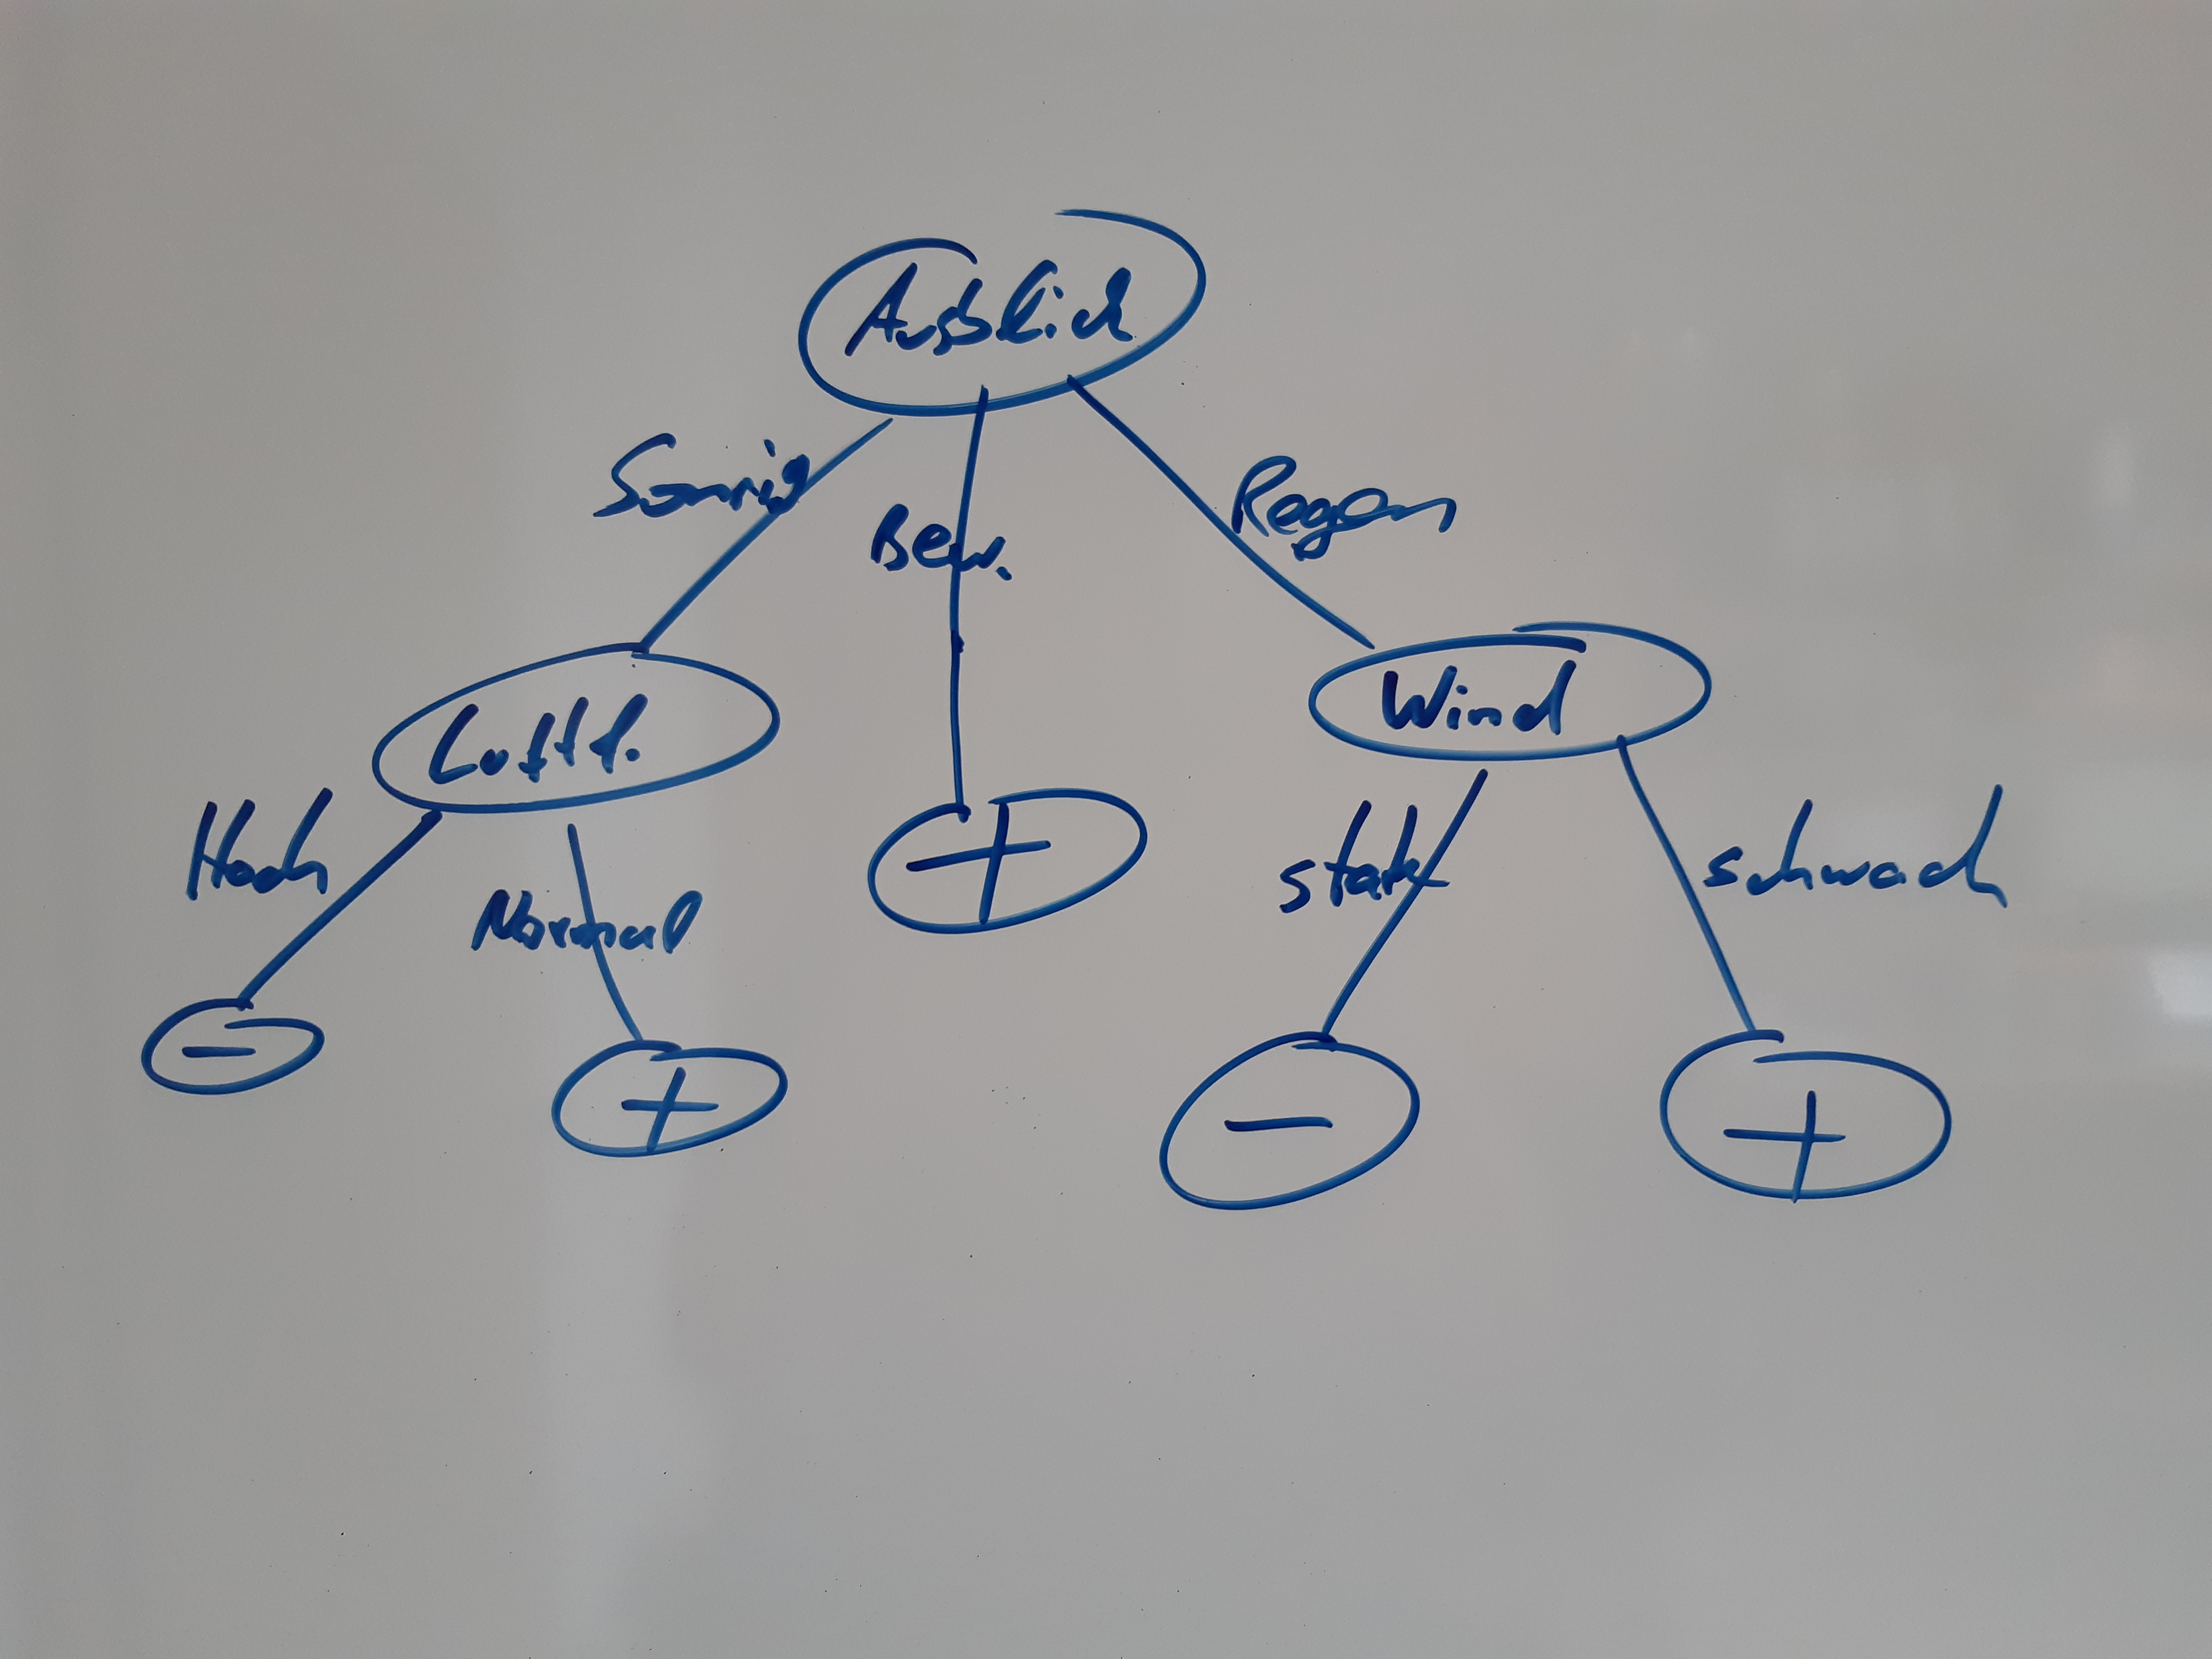
\includegraphics[width=0.5\textwidth]{1a.jpg}
\end{figure}
\end{solution}

\end{subtask}

\begin{subtask}[points=3,title=Vorhersage]
Geben Sie anhand ihres Entscheidungsbaumes eine Vorhersage für die Tage 15 bis 17 aus Tabelle~\ref{tab:data_baseball_predict}, ob Baseball gespielt wird.

\begin{solution}
Wenn wir dem erlernten Entscheidungsbaum folgen, ergibt sich
\begin{table}[h!]
	\centering
	\begin{tabular}{l|c|c|c|c|c}
		\toprule
		\textbf{Tag} & \textbf{Ausblick (A)} & \textbf{Temperatur (T)}  & \textbf{Luftfeuchtigkeit (L)} & \textbf{Wind (W)}     & \textbf{Spielt Baseball (B)} \\
		\midrule
		T15 & Sonnig    & Mild        & Hoch     & Schwach & -       \\
		T16 & Bewölkung & Mild        & Normal   & Schwach & +       \\
		T17 & Regen     & Kühl        & Normal   & Stark   & -       \\
		\bottomrule
	\end{tabular}
\end{table}
\newline
Wir spielen also nur an Tag 16.
\end{solution}

\end{subtask}
\end{task}
\newpage
\begin{task}[credit=4]{\codesym~Entscheidungsbäume - Klassifikation}
\label{t:dt_classification}
Im Institut Institut für Produktionstechnik und Umformmaschinen, kurz PtU\footnote{\url{https://www.ptu.tu-darmstadt.de/}}, der TU Darmstadt gibt es die Aufgabe eines Scherschneideverfahrens. Dabei wird mit Hilfe eines Stempels ein Loch in einen metallischen Werkstoff gestanzt, siehe Abbildung~\ref{fig:shearcutting}. Es gibt zwei Werkstoffe im Versuch: \texttt{CuSn6} und \texttt{16MnCr5}. Die Dicke des Materials beträgt entweder $0.4$\,mm oder $0.5$\,mm. Die Geschwindigkeit des Stempels liegt in den drei Stufen $100$, $200$ und $300$ vor.

\begin{figure}[h!]{
  \begin{minipage}{0.45\linewidth}
  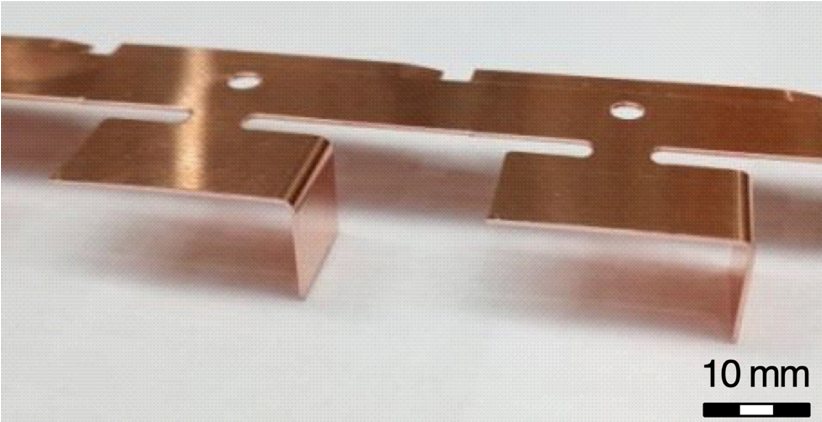
\includegraphics[width=\linewidth]{media/images/example.png}
  \end{minipage}
  \begin{minipage}{0.45\linewidth}
  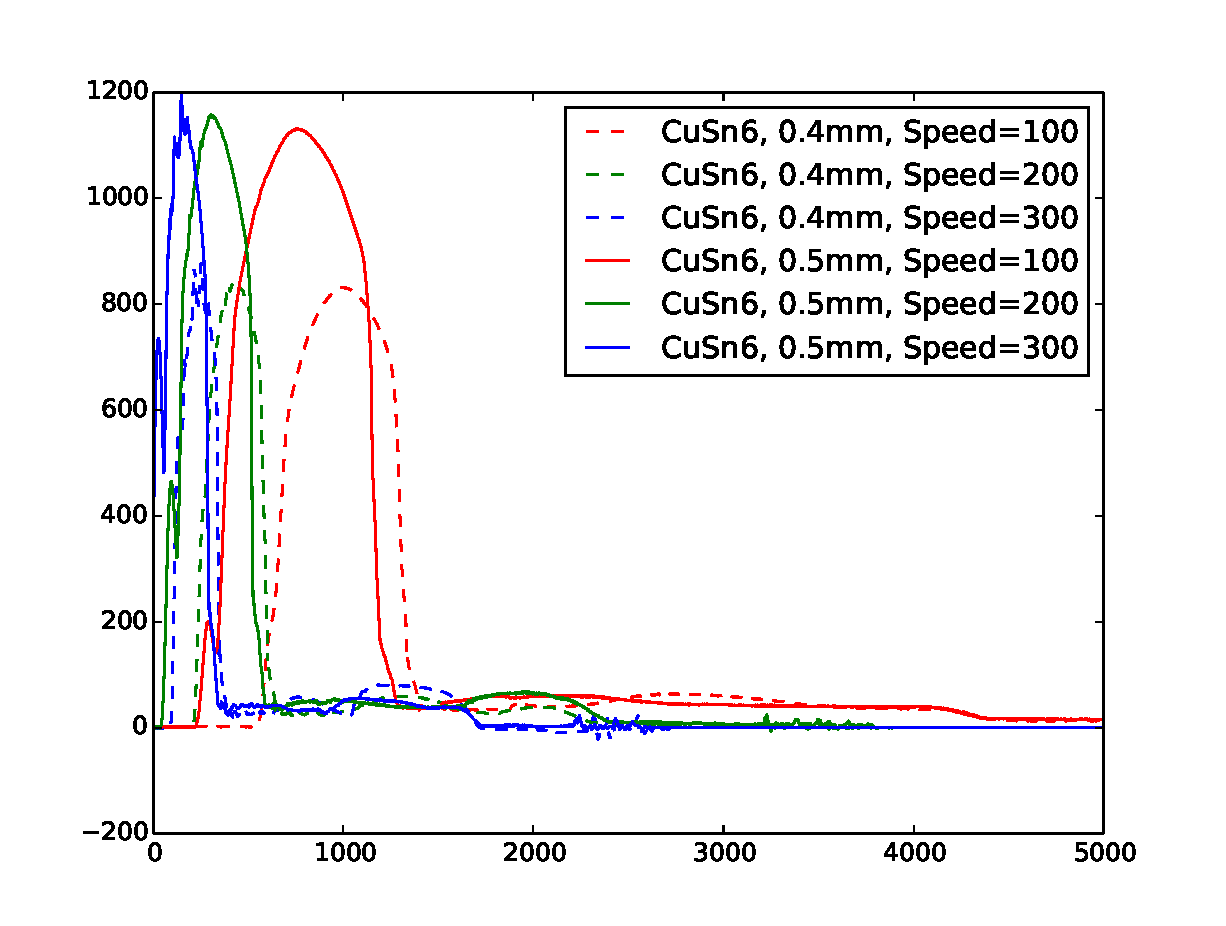
\includegraphics[width=\linewidth]{media/images/signal.pdf}%
  \end{minipage}}
  \caption{Links: Veranschaulichung des PtU Prozess. Rechts: Beispiel des Kraftsignals.}
  \label{fig:shearcutting}
 \end{figure}
 
Es gibt mehrere Sensoren, die den Status des Stanzen messen:

\begin{itemize}
 \item Kraft Sensor / Force sensor (Fz) 
 \item Verschiebungssensor / Displacement sensor (w)
 \item Beschleunigungssensor / Acceleration sensor (acc)
\end{itemize}
Im Experiment messen die Sensoren den Status des Stanzen von Beginn bis Ende jedes Prozesses.
Die Zeitreihendaten von jedem Sensor werden als 1D-Vektor dargestellt.
Das Interessante an dieser Aufgabe ist, dass der Status des Stanzen von der Art und Dicke des Materials abhängt. Andererseits ist es uns möglich, aus den Zeitreiheninformationen von den Sensoren auf die Art und Dicke des Materials und die Geschwindigkeit des Stanzen zu schließen.

\begin{itemize}
    \item \textbf{\texttt{Filename\_Fz\_raw.csv}}: Enthält Daten aus dem Kraftsensor. Jeder Zeilenvektor repräsentiert das Kraftsignal. Die Anzahl der Zeilen in der Datei beträgt $2787$, was der Anzahl der Experimente im Datensatz entspricht.
    \item \textbf{\texttt{Filename\_Speed.csv}}: Enthält die Geschwindigkeit des Schlags der $2787$ Proben.
    \item \textbf{\texttt{Filename\_thickness.csv}}: Enthält die Materialstärke der $2787$ Proben.
\end{itemize}

In dieser Übung verwenden wir die Daten des Kraftsensors, um die Proben nach der Geschwindigkeit des Stempels zu klassifizieren.

\begin{subtask}[points=3,title={\codesym~\texttt{02\_dt\_classification.py}}]
\label{t:dt_class}
Laden Sie die Daten des Kraftsensor aus \texttt{Filename\_Fz\_raw.csv} und die Geschwindigkeit des Stanzen aus \texttt{Filename\_Speed.csv} und vervollständigen Sie den Code in \texttt{02\_dt\_classification.py}:

\begin{itemize}
 \item[\codesym] Trainieren Sie einen Entscheidungsbaum zur Klassifikation in der Methode \texttt{fit\_dt\_classifier()} mithilfe von \texttt{sklearn} unter der Verwendung der Standardparameter.
 \item[\codesym] Ermitteln Sie die Testgenauigkeit in der Methode \texttt{get\_test\_accuracy()}.\\
 \item[\codesym] Plotten Sie den resultierenden Entscheidungsbaum in \texttt{export\_tree\_plot()}. Sie können dabei die Funktion \texttt{tree.export\_graphviz()} verwenden.
\end{itemize}
\end{subtask}

 \begin{subtask}[points=1,title=Visualisierung]
Zeigen Sie die erstelle Visualisierung des Entscheidungsbaumes zur Klassifikation aus Unteraufgabe~\ref{t:dt_class}.

\begin{solution}
% Geben sie hier ihre Antwort an.
\end{solution}

\end{subtask}
\end{task}


\begin{task}[credit=3]{Entscheidungsbäume - Regression}
Ein Entscheidungsbaum zur Regression kann auf den PtU Datensatz (s. Abb.~\ref{fig:shearcutting}) angewendet werden, um auf die Dicke des Materials zu schließen, welche ein kontinuierlicher Wert ist. 

 \begin{subtask}[points=2,title=\codesym~\texttt{03\_dt\_regression.py}]
 \label{t:dt_reg}
 Laden Sie die Daten des Kraftsensor aus \texttt{Filename\_Fz\_raw.csv} und die Materialstärken aus \texttt{Filename\_thickness.csv} und vervollständigen Sie den Code in \texttt{03\_dt\_regression.py}:
 
\begin{itemize}
    \item[\codesym] Trainieren Sie einen Entscheidungsbaum zur Regression in \texttt{fit\_dt\_regressor()}.
    \item[\codesym] Berechnen Sie den mittleren quadratischen Fehler für den Testdatensatz in der Funktion \texttt{get\_test\_mse()}.
\end{itemize}
\end{subtask}

 \begin{subtask}[points=1,title=Visualisierung]
Zeigen Sie die erstelle Visualisierung des Entscheidungsbaumes zur Regression aus Unteraufgabe~\ref{t:dt_reg}.

\begin{solution}
	Es ergab sich der folgende Entscheidungsbaum:
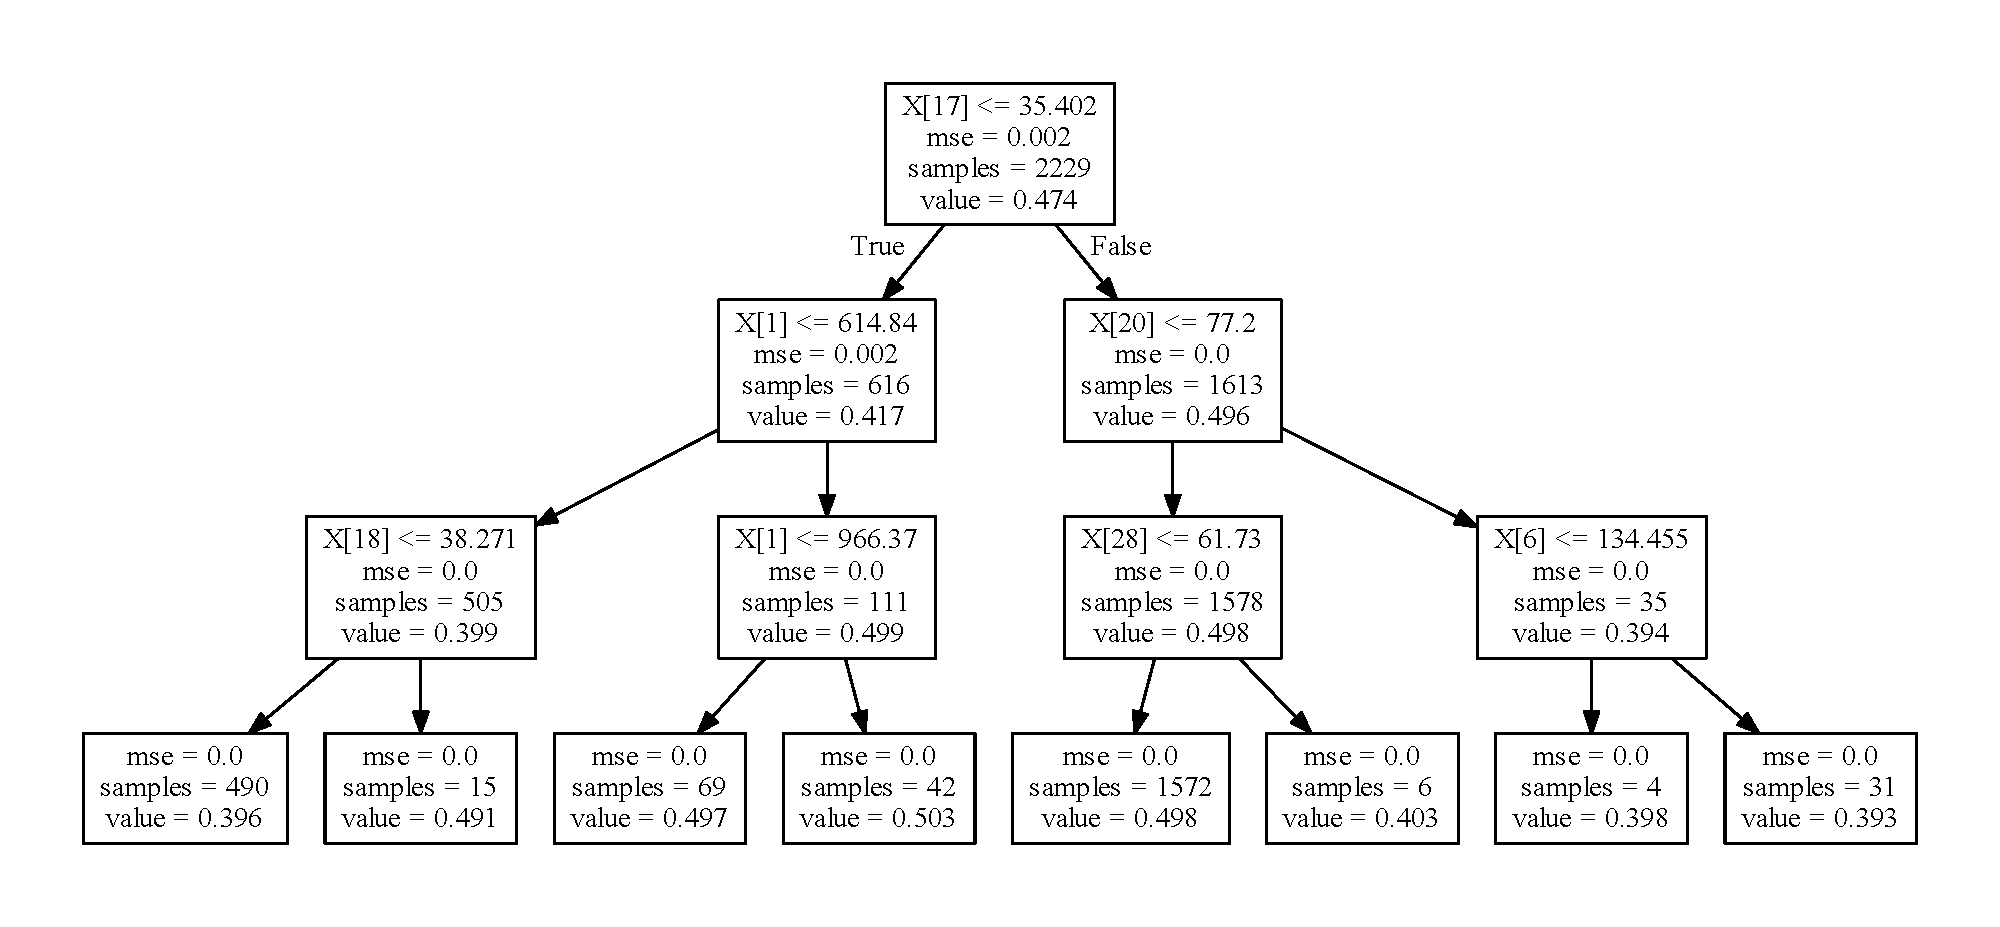
\includegraphics[width=\linewidth]{regression_tree_d3.pdf}
\end{solution}

\end{subtask}
\end{task}

\begin{task}[credit=4]{\codesym~Zufallswälder}
In dieser Aufgabe verwenden wir den PtU Datensatz (s. Abb.~\ref{fig:shearcutting}), um mit einem Zufallswald (engl. Random Forest) die Geschwindigkeit des Einschlags aus den Zeitreihen zu klassifizieren.
 
\begin{subtask}[points=2,title=\codesym~\texttt{04\_random\_forest.py}]
Laden Sie die Daten des Kraftsensor aus \texttt{Filename\_Fz\_raw.csv} und die Geschwindigkeit des Stanzen aus \texttt{Filename\_Speed.csv} und vervollständigen Sie den Code in \texttt{04\_random\_forest.py}:

\begin{itemize}
\item[\codesym] Trainieren Sie einen Zufallswald aus $100$ Entscheidungsstümpfen in der Methode \texttt{fit\_tree\_stump\_forest()}.

\item[\codesym] Trainieren Sie einen einzelnen Entscheidungsstumpf in der Methode \texttt{fit\_tree\_stump()}.
\end{itemize}
\end{subtask}

\begin{subtask}[title=Konfusionsmatrix,points=2]
Geben Sie die Konfusionsmatrizen des Trainings- und Testdatensatzes mit absoluten Werten für den Zufallswald  an.

\begin{solution}
	Es ergab sich für den Trainingsdatensatz die confusion matrix:
		\begin{table}[H]
			\begin{tabular}{lll}
				658 & 0   & 0   \\
				0   & 831 & 0   \\
				11  & 6   & 723
			\end{tabular}
		\end{table}
	und für den Testdatensatz:
		\begin{table}[H]
			\begin{tabular}{lll}
				166 & 0   & 0   \\
				0   & 207 & 0   \\
				2   & 4   & 179
			\end{tabular}
		\end{table}
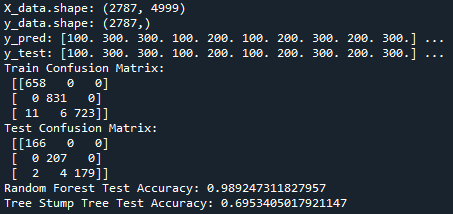
\includegraphics[width=\linewidth]{ue4ergebnisse.png}
\end{solution}

\end{subtask}

\end{task}

\newpage
\begin{task}[credit=15]{AdaBoost}
In dieser Aufgabe werden Sie AdaBoost auf die gegebenen Trainingsbeispiele aus der Tabelle~\ref{t:boost_data} anwenden. 

\begin{table}[h]
\caption{Datensatz mit zwei Merkmalen und zwei Zielklassen.}
\label{t:boost_data}
\centering
\begin{tabular}{c|c|c}
$\mathbf{x_1}$ & $\mathbf{x_2}$  & \textbf{Klasse} \\
\midrule
1 & 5  & +      \\
2 & 2  & +      \\
5 & 8  & +      \\
6 & 10 & +      \\
8 & 7  & +      \\
3  & 1 & -      \\
4  & 6  & -     \\
7  & 4  & -     \\
9  & 3  & -     \\
10 & 9  & -     \\
\bottomrule
\end{tabular}
\end{table}

Entscheidungsstümpfe mit ganzzahligem Schwellwert (z.B. $\mathbf{x_1}\leq T \Rightarrow +$ oder $\mathbf{x_1} > T \Rightarrow +$) sollen als Basis-Lerner verwendet werden. Der Basis-Lerner minimiert die Summe der Gewichtungen der falsch klassifizierten Beispiele aus allen möglichen Aufteilungen. Für ein Unentschieden wählen Sie die erste gefundene Übereinstimmung, beginnend mit Entscheidungsstümpfen für $\mathbf{x_1}$ und dann $\mathbf{x_2}$.

Verwenden Sie die Formel:
\begin{equation}
    \alpha_{i} = \frac{1}{2}\log\left (\frac{1-err_{i}}{err_{i}}\right )
\end{equation}
zur Berechnung von $\alpha_{i}$.

\begin{subtask}[title=Algorithmus,points=12]
 Zeigen Sie die Ausführung des Adaboost Algorithmus für die \textbf{ersten beiden} Iterationen.
 Geben Sie dabei die \textbf{Fehler} (Summe der Gewichtungen der falsch klassifizierten Beispiele) für die möglichen Entscheidungsgrenzen von $1$ bis $10$ an, sowie die \textbf{Gewichtung} jedes Datenpunktes vor und nach Normalisierung an.

\begin{solution}
\begin{table}[h]
	\centering
	\begin{tabular}{ll|rr|rrrrrr}
		Kriterium & Entscheidung & erste & Iteration &  & zweite &  & Iteration & & \\
		\hline
		& & Fehler $x_1$ & Fehler $x_2$ & $x_1$ schlecht & $x_1$ gut& Fehler $x_1$ & $x_2$ schlecht & $x_2$ gut & Fehler $x_2$ \\
		$x_i \leq 0$ & pro + & 0.5 & 0.5 & 3 &2 & 0.5821 & 3 &2 & 0.5821\\
		$x_i \leq 0$ & pro - & 0.5 & 0.5 & 0 &5 & 0.4315 & 0 &5 & 0.4315\\
		$x_i \leq 1$ & pro + & 0.4 & 0.6 & 3 &1 & 0.4958 & 3 &3 & 0.6684 \\
		$x_i \leq 1$ & pro - & 0.6 & 0.4 & 0 &6 & 0.5178 & 0 &4 & 0.3452 \\
		$x_i \leq 2$ & pro + & \fbox{0.3} & 0.5 & 3 &0 & 0.4095 & 3 &2 & 0.5821 \\
		$x_i \leq 2$ & pro - & 0.7 & 0.5 & 0 &7 & 0.6041 & 0 &5 & 0.4315\\
		
		$x_i \leq 3$ & pro + & 0.4 & 0.6 & 3 &1 & 0.4958 & 3 &3 & 0.6684 \\
		$x_i \leq 3$ & pro - & 0.6 & 0.4 & 0 &6 & 0.5178 & 0 &4 & 0.3452\\
		
		$x_i \leq 4$ & pro + & 0.5 & 0.7 & 3 &2 & 0.5821 & 3 &4 & 0.7547 \\
		$x_i \leq 4$ & pro - & 0.5 & 0.3 & 0 &5 & 0.4315 & 0 &3 & 0.2589 \\
		
		$x_i \leq 5$ & pro + & 0.4 & 0.6 & 2 &2 & 0.4456 & 3 &3 & 0.6684 \\
		$x_i \leq 5$ & pro - & 0.6 & 0.4 & 1 &5 & 0.568  & 0 &4 & 0.3452 \\
		
		$x_i \leq 6$ & pro + & 0.3 & 0.7 & 1 &2 & 0.3091 & 3 &4 & 0.7547 \\
		$x_i \leq 6$ & pro - & 0.7 & 0.3 & 2 &5 & 0.7045 & 0 &3 & 0.2589 \\
		
		$x_i \leq 7$ & pro + & 0.4 & 0.6 & 1 &3 & 0.3954 & 2 &4 & 0.6182 \\
		$x_i \leq 7$ & pro - & 0.6 & 0.4 & 2 &4 & 0.6182 & 1 &3 & 0.3954 \\
		
		$x_i \leq 8$ & pro + & 0.3 & 0.5 & 0 &3 & \fbox{0.2589} & 1 &4& 0.4817 \\
		$x_i \leq 8$ & pro - & 0.7 & 0.5 & 3 &4 & 0.7547 & 2 &3 & 0.5319 \\
		
		$x_i \leq 9$ & pro + & 0.4 & 0.6 & 0 &4 &0.3452 & 1 &5& 0.568 \\
		$x_i \leq 9$ & pro - & 0.6 & 0.4 & 3 &3 & 0.6684 & 2 &2 & 0.4456 \\
		
		$x_i \leq 10$ & pro + & 0.5 & 0.5 & 0 &5 & 0.4315 & 0 &5 & 0.4315 \\
		$x_i \leq 10$ & pro - & 0.5 & 0.5 & 3 &2 & 0.5821 & 3 &2 & 0.5821 \\
		
	\end{tabular}
	\caption{Die Ergebnisse für Aufgabe 1.5. Die Tabelle liest sich am Beispiel der Zeile 3 folgendermaßen: entscheiden wir uns bei $x_1 \leq 1$ für + dann machen wir 4 Fehler im ersten Schritt (also Fehlermaß 0.4) und 3 schlechte (d.h. höher gewichtete) Fehler bzw. einen guten (d.h. niedriger gewichteten) im zweiten Schritt. Daraus errechnet sich das Fehlermaß. Entscheiden wir uns bei $x_2 \leq 1$ für +, dann machen wir 6 Fehler im ersten Schritt und sowohl 3 schlechte als auch 3 gute im zweiten Schritt. Daraus ergibt sich dann das Fehlermaß.  }
	\label{tab:H1.5-Ergebnis}
\end{table}	
Im ersten Schritt gilt für alle Gewichte $w_i = 0.1$, für $i = 1, \ldots, 10$. Also müssen wir nur zählen, wie viele falsch klassifiziert werden. Betrachte dazu Spalten 3 und 4 in Tabelle \ref{tab:H1.5-Ergebnis}. Da wir bei einem Unentschieden das erste Minimum beginnend mit $x_1$ wählen sollen, gilt \begin{align*}
f_1 ((x_1, x_2)^T) = \left\{
\begin{array}{ll}
+1 & x_1 \leq 2 \\
-1 & \, \textrm{sonst} \\
\end{array}
\right. 
\end{align*} als Stumpf für die erste Iteration. Damit gilt nach Zeile 5 der Tabelle \ref{tab:H1.5-Ergebnis} $err_1 = 0.3$. Weiter ist \begin{align*}
\alpha_1 = \frac{1}{2}ln(\frac{1-err_1}{err_1}) = 0.4236.
\end{align*} Behalten wir die Nummerierung in der Aufgabenstellung bei (beginnend bei 1), dann klassifizieren wir die Punkte 3, 4 und 5 falsch. Dementsprechend erhalten wir für die neuen (noch nicht normalisierten) Gewichte \begin{align*}
w_i' &= 0.1 \text{ für } i = 1,2,6,7,8,9,10 \\
w_i' &= 0.1e^{\alpha_1} = 0.1527 \text{ für } i = 3,4,5.
\end{align*} Normalisieren (d.h. teilen durch 7 * 0.1 + 0.1527 * 3= 1.1581) ergibt \begin{align*}
w_i^{(1)} &= 0.0863 \text{ für } i = 1,2,6,7,8,9,10 \\
w_i^{(1)} &= 0.1365 \text{ für } i = 3,4,5.
\end{align*} Für den zweiten Iterationsschritt müssen wir darauf achten, dass die Datenpunkte 3, 4 und 5 stärker gewichtet sind, wir also eine erneute Fehlklassifikation vermeiden sollten. Der zu minimierende Fehler ist \begin{align*}
0.0863(\epsilon_1 + \epsilon_2 +\epsilon_3 +\epsilon_4 +\epsilon_8 +\epsilon_9 +\epsilon_{10} ) + 0.1365(\epsilon_5 +\epsilon_6 +\epsilon_7)
\end{align*}wobei \begin{align*}
\epsilon_i = \left\{\begin{array}{ll}
1 & \text{Datenpunkt i wurde falsch klassifiziert} \\
0 & \text{Datenpunkt i wurde korrekt klassifiziert} \\
\end{array} 
\right.
\end{align*} gilt. Aus Spalte 7 in Tabelle \ref{tab:H1.5-Ergebnis} ersehen wir, dass der neue Rumpf \begin{align*}
f_2 ((x_1, x_2)^T) = \left\{
\begin{array}{ll}
+1 & x_1 \leq 8 \\
-1 & \, \textrm{sonst} \\
\end{array}
\right. 
\end{align*} ist. Es gilt $err_2 = 3 * 0.0863 = 0.2589$ und wir klassifizieren die Datenpunkte 6, 7 und 8 falsch. Es folgt \begin{align*}
\alpha_2 = \frac{1}{2}ln(\frac{1-err_2}{err_2}) = 0.5258.
\end{align*} Wir müssen die Datenpunkte 6, 7 und 8 neu gewichten, also \begin{align*}
w_i' &= 0.1 * e^{0.5258} = 0.1692 \text{ für } i = 6,7,8 \\
w_i' &= 0.0863 \text{ für } i = 1,2,9,10 \\
w_i' &= 0.1365 \text{ für } i = 3,4,5.
\end{align*} mit. Nach Normalisierung (d.h. teilen durch 3 * 0.1365 + 3 * 0.1692 + 4 * 0.0863 = 1.2623) folgt \begin{align*}
w_i^{(2)} &= 0.1081 \text{ für } i = 3,4,5 \\
w_i^{(2)} &= 0.1340 \text{ für } i = 6,7,8 \\
w_i^{(2)} &= 0.0684 \text{ für } i = 1,2,9,10 
\end{align*}

\end{solution}

\end{subtask}

\begin{subtask}[title=Gesamtmodell,points=3]
 Geben Sie das Gesamtmodell $f(x)$ nach zwei Iterationen an.
 
\begin{solution}
Mit der Notation aus Teilaufgabe a) folgt mit $x = (x_1, x_2)^T \in \mathbb{R}^2$ \begin{align*}
\tilde{f}(x) = \alpha_1f_1(x) + \alpha_2f_2(x) = \left\{
\begin{array}{ll}
0.9494 & x_1 \leq 2 \\
0.1022 & 2 < x_1 \leq 8 \\
-0.9494 & x_1 > 8 
\end{array}
\right. 
\end{align*} Für das Gesamtmodell nach zwei Iterationen ergibt sich also \begin{align*}
f(x) = sign(\tilde{f}(x)) = \left\{
\begin{array}{ll}
1 &  x_1 \leq 8 \\
-1 & x_1 > 8 
\end{array}
\right. 
\end{align*}
\end{solution}

\end{subtask}

\end{task}


\newpage
%\section{Aufgabe: Naive Bayes}
\begin{task}[credit=19]{Na\"ive Bayes}
In dieser Aufgabe verwenden wir wieder den Baseball-Datensatz (s. Tabelle~\ref{tab:data_baseball} und 2) und einen Na\"ive Bayes Klassifikator, um zu entscheiden ob Baseball gespielt wird oder nicht.
\begin{comment}
\begin{table}[h!]
\centering
\begin{tabular}{|l|l|l|l|l|l|}
\hline
Day & Outlook  & Temperature & Humidity & Wind   & Play ball \\ \hline
D1  & Sunny    & Hot         & High     & Weak   & No        \\ \hline
D2  & Sunny    & Hot         & High     & Strong & No        \\ \hline
D3  & Overcast & Hot         & High     & Weak   & Yes       \\ \hline
D4  & Rain     & Mild        & High     & Weak   & Yes       \\ \hline
D5  & Rain     & Cool        & Normal   & Weak   & Yes       \\ \hline
D6  & Rain     & Cool        & Normal   & Strong & No        \\ \hline
D7  & Overcast & Cool        & Normal   & Strong & Yes       \\ \hline
D8  & Sunny    & Mild        & High     & Weak   & No        \\ \hline
D9  & Sunny    & Cool        & Normal   & Weak   & Yes       \\ \hline
D10 & Rain     & Mild        & Normal   & Weak   & Yes       \\ \hline
D11 & Sunny    & Mild        & Normal   & Strong & Yes       \\ \hline
D12 & Overcast & Mild        & High     & Strong & Yes       \\ \hline
D13 & Overcast & Hot         & Normal   & Weak   & Yes       \\ \hline
D14 & Rain     & Mild        & High     & Strong & No        \\ \hline
\end{tabular}
\caption{Training data}
\end{table}
\end{comment}


\begin{subtask}[title={Formel für Merkmalsausprägung},points=4]
Zeigen Sie die Formel für $P(B=Ja \mid Merkmal)$ und  $P(B=Nein \mid Merkmal) $ für den gegebenen Datensatz.

\begin{solution}
Sei Merkmal = (Ausblick, Temperatur, Luftfeuchtigkeit, Wind) ein 4-Tupel aus Untermerkmalen. Dabei kürzen wir Ausblick mit A, Temperatur mit T, Luftfeuchtigkeit mit T und Wind mit W ab. Zur besseren Lesbarkeit sei weiterhin N := 'B = Nein', J := 'B = Ja'. Nach der Unabhängigkeitsannahme des Naive Bayes-Ansatzes gilt \begin{align*}
p(Merkmal|J) &= p(A|J)\cdot p(T|J)\cdot p(L|J)\cdot p(W|J) \text{ und } \\
p(Merkmal|N) &= p(A|N)\cdot p(T|N)\cdot p(L|N)\cdot p(W|N).
\end{align*} Damit können wir rechnen \begin{align*}
p(J|Merkmal) &= \frac{p(Merkmal|J)\cdot p(J)}{p(Merkmal)} \\
&= \frac{p(Merkmal|J)\cdot p(J)}{p(Merkmal|J)\cdot p(J) + p(Merkmal|N)\cdot p(N) } \\ &= \frac{ p(A|J)\cdot p(T|J)\cdot p(L|J)\cdot p(W|J)\cdot p(J)}{p(A|J)\cdot p(T|J)\cdot p(L|J)\cdot p(W|J)\cdot p(J) +  p(A|N)\cdot p(T|N)\cdot p(L|N)\cdot p(W|N)\cdot p(N) }.
\end{align*} Die erste Gleichheit ist der Satz von Bayes, die zweite die Formel der totalen Wahrscheinlichkeit und die dritte die Unabhängigkeitsannahme von oben. Völlig analog gilt \begin{align*}
p(N|Merkmal) &= \frac{p(Merkmal|N)\cdot p(N)}{p(Merkmal)} \\
&= \frac{p(Merkmal|N)\cdot p(N)}{p(Merkmal|J)\cdot p(J) + p(Merkmal|N)\cdot p(N) } \\ &= \frac{ p(A|N)\cdot p(T|N)\cdot p(L|N)\cdot p(W|N)\cdot p(N)}{p(A|J)\cdot p(T|J)\cdot p(L|J)\cdot p(W|J)\cdot p(J) +  p(A|N)\cdot p(T|N)\cdot p(L|N)\cdot p(W|N)\cdot p(N) }.
\end{align*}
\end{solution}

\end{subtask}
 
\begin{subtask}[title=Wahrscheinlichkeiten,points=6]
Bestimmen Sie angesichts der oben genannten Trainingsdaten alle Wahrscheinlichkeiten, die erforderlich sind, um den Na\"ive Bayes Klassifikator für beliebige Vorhersagen, ob Baseball gespielt wird, anzuwenden.

\begin{solution}
Wir kürzen die Begriffe wie folgt ab: Sonnig - S, Regen - R, Bewölkung - B; Warm - W, Mild - M, Kühl - K; Hoch - H, Normal - No; Schwach - Sch, Stark - St. Durch einfaches Auszählen ergibt sich p(B = Ja) = 9/14, p(B = Nein) = 5/14 sowie
\begin{tabular}{l|l|l|l}
	Ausblick & Temperatur & Luftfeuchtigkeit & Wind \\ \hline
p(A = S) = 5/14 & p(T = W) = 4/14 & p(L = H) = 7/14 & p(W = Sch) = 8/14 \\
p(A = R) = 5/14 & p(T = M) = 6/14 & p(L = No) = 7/14 & p(W = St) = 6/14 \\
p(A = B) = 4/14 & p(T = K) = 4/14 &                 &                    \\ 
p(A = S|Ja) = 2/9 & p(T = W|Ja) = 2/9 & p(L = H|Ja) = 3/9 & p(W = Sch|Ja) = 6/9 \\
p(A = B|Ja) = 4/9 & p(T = M|Ja) = 4/9 & p(L = No|Ja) = 6/9 & p(W = St| Ja) = 3/9 \\
p(A = R|Ja) = 3/9 & p(T = K|Ja) = 3/9 &                   &                     \\ 
p(A = S|Nein) = 3/5 & p(T = W|Nein) = 2/5 & p(L = H|Nein) = 4/5 & p(W = Sch|Nein) = 2/5 \\
p(A = B|Nein) = 0/5 & p(T = M|Nein) = 2/5 & p(L = No|Nein) = 1/5 & p(W = St|Nein) = 3/5  \\
p(A = R|Nein) = 2/5 & p(T = K|Nein) = 1/5 &                     &                       
\end{tabular} 
\end{solution}

\end{subtask}

\begin{subtask}[points=9,title=Vorhersage]
Treffen Sie Vorhersagen nach Na\"ive Bayes für die Tage 15 bis 17 aus Tabelle~\ref{tab:data_baseball_predict}, ob Baseball gespielt wird.
Geben Sie dabei den Rechenweg an.

\begin{solution}
Wir setzen die Zahlen aus b) in die Formel von a) ein und erhalten für Tag 15\begin{align*}
 p(B = Ja| S, M, H, Sch) &= \frac{p(S|Ja)p(M|Ja)p(H|Ja)p(Sch|Ja)p(Ja)}{p(S|Ja)p(M|Ja)p(H|Ja)p(Sch|Ja)p(Ja) + p(S|N)p(M|N)p(H|N)p(Sch|N)p(N)} \\
&= \frac{2/9\cdot4/9\cdot3/9\cdot6/9\cdot9/14}{2/9\cdot4/9\cdot3/9\cdot6/9\cdot9/14 + 3/5\cdot2/5\cdot4/5\cdot2/5\cdot5/14} = \frac{8/567}{8/567 + 24/875} = 0,33967.
\end{align*} Es folgt $p(B = Nein| S, M, H, Sch) = 1- p(B = Ja| S, M, H, Sch) = 0.66 > 0.5$, sodass an Tag 15 kein Baseball gespielt wird. Tag 16: \begin{align*}
p(B = Ja| B, M, No, Sch) &= \frac{p(B|Ja)p(M|Ja)p(No|Ja)p(Sch|Ja)p(Ja)}{p(B|Ja)p(M|Ja)p(No|Ja)p(Sch|Ja)p(Ja) + p(B|N)p(M|N)p(No|N)p(Sch|N)p(N)} \\ &= \frac{4/9\cdot4/9\cdot6/9\cdot6/9\cdot9/14}{4/9\cdot4/9\cdot6/9\cdot6/9\cdot9/14 + 0/5\cdot2/5\cdot1/5\cdot2/5\cdot5/14} = 1,
\end{align*} also wird an Tag 16 Baseball gespielt. \\ Für Tag 17 ergibt sich \begin{align*}
p(B = Ja| R, K, No, St) &= \frac{p(R|Ja)p(K|Ja)p(No|Ja)p(St|Ja)p(Ja)}{p(R|Ja)p(K|Ja)p(No|Ja)p(St|Ja)p(Ja) + p(R|N)p(K|N)p(No|N)p(St|N)p(N)} \\
&= \frac{3/9\cdot3/9\cdot6/9\cdot3/9\cdot9/14}{3/9\cdot3/9\cdot6/9\cdot3/9\cdot9/14 + 2/5\cdot1/5\cdot1/5\cdot3/5\cdot5/14} = \frac{1/63}{1/63 + 3/875} = 0,822.
\end{align*} Somit wird an Tag 17 Baseball gespielt. 
\end{solution}

\end{subtask}
\end{task}

\newpage
\begin{task}[credit=6]{K-Means}

Folgender Datensatz besteht aus $8$ Punkten:
\begin{equation}
 \begin{aligned}
&x_1=(2,8), \quad x_2=(2,5),\quad x_3=(1,2), \quad x_4=(5,8),\\
&x_5=(7,3), \quad x_6=(6,4),\quad x_7=(8,4), \quad x_8=(4,7).
 \end{aligned}
\end{equation}

\begin{figure}[h!]
\centering
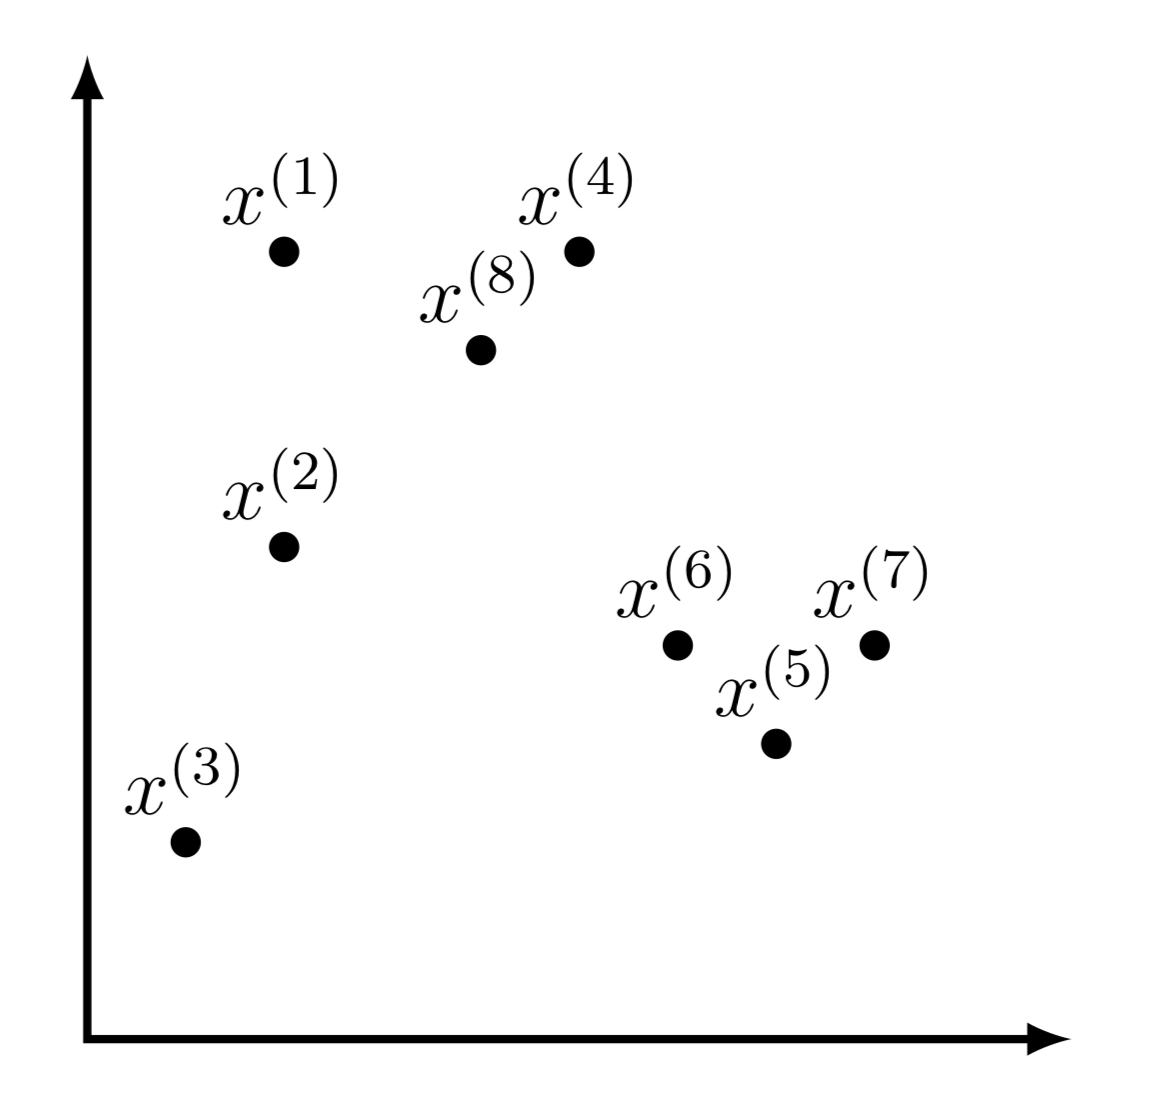
\includegraphics[width=0.4\linewidth]{media/images/kmeans.png}
\caption{Visualisierung des K-Means Datensatzes}
\end{figure}

\begin{subtask}[points=6,title={K-Means Algorithmus}]
Benutzen Sie den K-Means Algorithmus mit der Euklidischen Distanz um diese $8$ Datenpunkte in $K=3$ Cluster einzuteilen.
Nehmen Sie dabei an, dass die Clusterzentren mit den Punkten $x_2$, $x_4$ und $x_8$ initialisiert sind.
Führen Sie zwei Iterationen des K-Means Algorithmus durch und geben Sie die Koordinaten der Zentroide der Cluster an.

\begin{solution}
% Geben sie hier ihre Antwort an.
\end{solution}

\end{subtask}

\end{task}


\newpage
\begin{task}[credit=7]{Regressionsanalyse}
Gegeben sind folgende Datenpunkte:

\begin{table}[h]
\centering
\begin{tabular}{c|cccccccc}
\toprule
\textbf{x} & 1 & 3 & 4 & 6 & 8 & 9 & 11 & 14 \\ \hline
\textbf{y} & 1 & 2 & 4 & 4 & 5 & 7 & 8  & 9  \\
\bottomrule
\end{tabular}
\end{table}

\begin{figure}[h]
\centering
\caption{Veranschaulichung der Datenpunkte zur linearen Regression.}
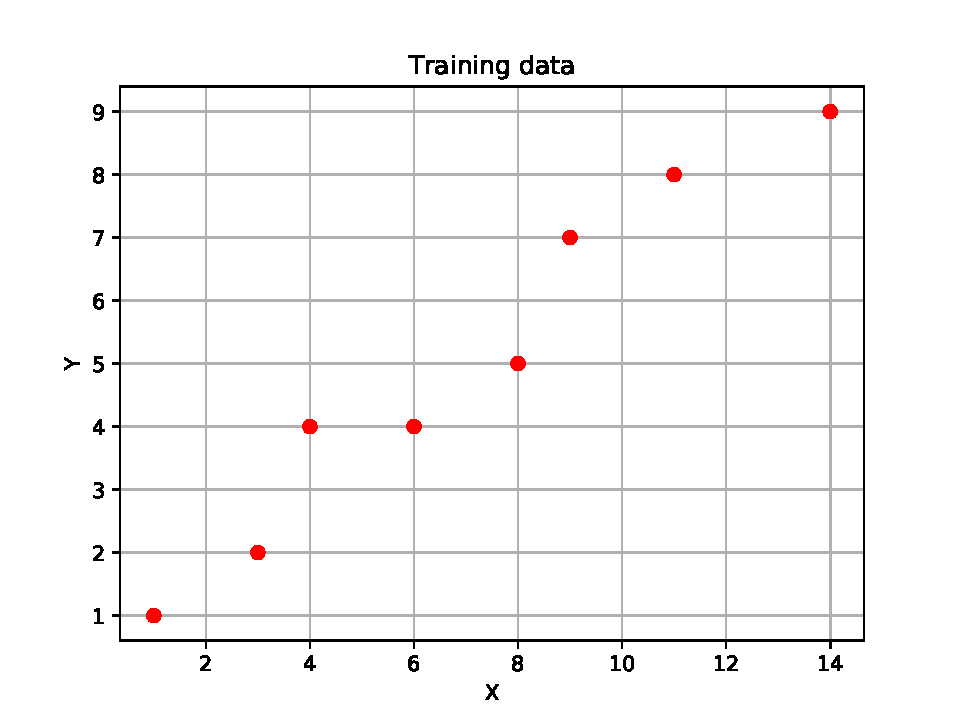
\includegraphics[width=0.5\linewidth]{media/images/data.pdf}
\end{figure}

%We want to build a least square regression model 
Wir möchten eine Regression nach dem Prinzip der kleinsten Fehlerequadrate erstellen:

\begin{equation}
y =f(x)=\left \langle W, x  \right \rangle+b\,.
\end{equation}

Mit der Hilfe eines $(p+1)$-dimensionalen Vektors $\vec{x}=(1, x_1, \cdots , x_p)$ und $x \in \mathbb{R}^{1 \times p}$, können wir $b$ in dem Vektor $W$ codieren:

\begin{equation}
y =f(x)=\left \langle W^{'}, \vec{x}^{T}  \right \rangle,
\end{equation}

wobei hier $W^{'} \in \mathbb{R}^{2 \times 1}$ und $\vec{x} \in \mathbb{R}^{1 \times 2}$.

\begin{subtask}[title=Herleitung,points=5]
 Zeigen Sie, dass das optimale $W^{'}$:
\begin{equation}
W^{'} =  (\vec{X}^{T}\vec{X})^{-1}\vec{X}^{T}Y,
\end{equation}
entspricht, wobei $\vec{X} \in \mathbb{R}^{n \times 2}$ und $Y \in \mathbb{R}^{n \times 1}$.

\begin{solution}
Wir möchten eine Regression nach dem Prinzip der kleinsten Fehlerquadrate erstellen. Das heißt wir wollen folgende Funktion minimieren:
\begin{align*}
\min_{W,b} S(W,b) = \sum_{i=1}^n (W^T x_i + b - y_i)^2.
\end{align*}
Dies ist nach den obigen Definitionen äquivalent zur Minimierung folgender Funktion:
\begin{align*}
\min_{W'} S(W') = \sum_{i=1}^n (W'^T \bar{x}_i - y_i)^2.
\end{align*}
Daraus folgt
\begin{align*}
S(W') &= \sum_{i=1}^n (W'^T \bar{x}_i - y_i)^2 = ||  \vec{X} W' - Y ||^2\\
&= (\vec{X}W' - Y)^T(\vec{X}W' - Y) \\
&= W'^T \vec{X}^T \vec{X}W' - Y^T \vec{X} W' - W'^T \vec{X}^T Y + Y^T Y \\
&= W'^T \vec{X}^T \vec{X} W' - 2 Y^T \vec{X} W' + Y^T Y
\end{align*}
Wir differenzieren nun die Funktion $S(W')$ nach $W'$
\begin{align*}
\frac{\partial S(W')}{\partial W'} &= 2 W'^T \vec{X}^T \vec{X} - 2 Y^T \vec{X}.
\end{align*}
Setzen wir die Ableitung gleich 0 erhalten wir
\begin{align*}
0 &= W'^T \vec{X}^T \vec{X} - Y^T \vec{X} \\
W'^T \vec{X}^T \vec{X} &= Y^T \vec{X} \\
\vec{X}^T \vec{X} W' &= \vec{X}^T Y \\
W' &= (\vec{X}^T \vec{X})^{-1} \vec{X}^T Y
\end{align*}
unter der Bedingung, dass die Inverse $(\vec{X}^T \vec{X})^{-1}$ existiert.
\end{solution}
\end{subtask}


\begin{subtask}[title=Parameterbestimmung,points=2]
Berechnen Sie $W$ und $b$ für den gegebenen Punktdatensatz. Die Inverse $(\vec{X}^{T}\vec{X})^{-1}$ muss dabei nicht manuell berechnet werden.

\begin{solution}
Durch ablesen der Koordinaten erhalten wir: 
\begin{align*}
\vec{X} = 
\begin{pmatrix}
1 & 1 \\
1 & 3 \\
1 & 4 \\
1 & 6 \\
1 & 8 \\
1 & 9 \\
1 & 11 \\
1 & 14 \\
\end{pmatrix}
\text{ und }
\vec{Y} = 
\begin{pmatrix}
1 \\
2 \\
4 \\
4 \\ 
5 \\
7 \\
8 \\ 
9 \\
\end{pmatrix}.
\end{align*}
Daraus folgt
\begin{align*}
\vec{X}^T \vec{X} = 
\begin{pmatrix}
8 & 56 \\
56 & 524 \\
\end{pmatrix}
\text{ und }
(\vec{X}^T \vec{X})^{-1} = 
\begin{pmatrix}
\frac{131}{264} & \frac{-7}{132} \\
\frac{-7}{132} & \frac{1}{132} \\
\end{pmatrix}
\end{align*}
Damit können wir nun W und b berechnen
\begin{align*}
W' &= 
\begin{pmatrix}
\frac{131}{264} & \frac{-7}{132} \\
\frac{-7}{132} & \frac{1}{132} \\
\end{pmatrix}
\begin{pmatrix}
40 \\
364 \\
\end{pmatrix} 
= (\vec{X}^T \vec{X})^{-1} \vec{X}^T Y \\
&= 
\begin{pmatrix}
\frac{6}{11}
\frac{7}{11}
\end{pmatrix}
\end{align*}
Daraus folgt $W= \frac{7}{11}$ und $b = \frac{6}{11}$.
\end{solution}

\end{subtask}
\end{task}


%\bibliography{library}{}
%\bibliographystyle{plain}

\end{document}
